\subsection{Modelo propuesto}

Se extrajeron las siguientes capas de la red MobileNet v2.

\begin{itemize}
    \item block\_1\_expand\_relu
    \item block\_3\_expand\_relu
    \item block\_6\_expand\_relu
    \item block\_13\_expand\_relu
    \item block\_16\_project
\end{itemize}

Las cuales seran usadas para realizar la concadenación con las capas de expansión. De igual manera se extrajeron las siguientes capas del modelo pix2pix.

\begin{itemize}
    \item  pix2pix.upsample(512, 3)
    \item pix2pix.upsample(256, 3)
    \item pix2pix.upsample(128, 3)
    \item pix2pix.upsample(64, 3)
\end{itemize}

Estas capas conformaran las capas de expansión del modelo U-Net. El modelo en su totalidad se encuentra ilustrado en la figura \ref{fig:model}.

\begin{figure}[H]
    \centering
    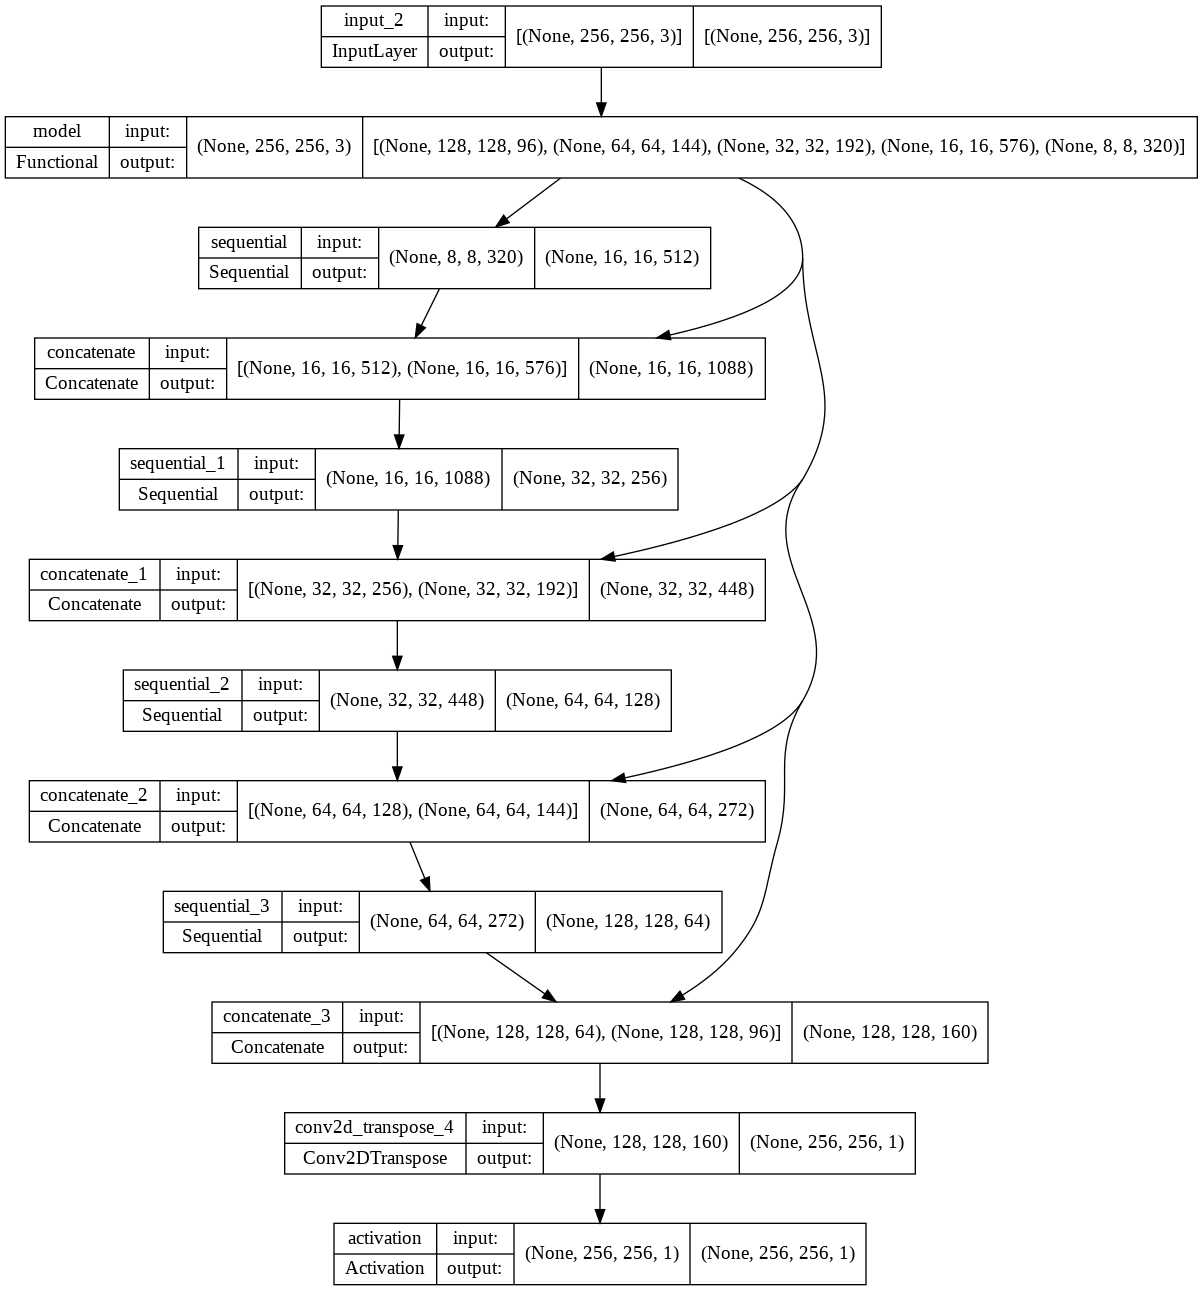
\includegraphics[width=12cm]{Graphics/model.png}
    \caption{Modelo usando capas de la red MobileNet v2 y pix2pix.}
    \label{fig:model}
\end{figure}

\subsection{Tipos de entrenamiento}

El modelo fue entrenado de diferentes estrategias. Eso para observar los tiempos de entrenamiento y los resultados que se obtienen con cada modelo.

\subsubsection{Conexion directa}

En este tipo de entrenamiento se congelaron los pesos de las capas extraidas de MobileNet v2.

\subsubsection{Fine tunning}

En este tipo de entrenamiento se descongelo unicamente la capa block\_16\_project del modelo MobileNet v2. Las demás se dejaron congeladas.

\subsubsection{Full tunning}

En este tipo de entrenamiento se descongelaron todas las capas extraidas de MobileNet v2.